\section{Bounding the Board}
\label{board_bound}

Let $G = (V, E)$ be a lattice graph. Following \cite{demaine} we define the \emph{potential of $G$}
\[
  \pot(G) = 8 \cdot \# V - 2 \cdot \# E.
\]
%We call $\pot(G)$ the . 
In this Section it will appear that the missing constraint which makes the original linear problem (\ref{lp0}---\ref{lp4}) accessible to modern LP solvers is an additional bound on the shape and potential of the board (see Theorem \ref{thm:octagonalization}), which in turn, thanks to  Lemma \ref{lem:octagons}, will imply a bound on the size of relevant boards. In order to formulate the bound we need some new geometric notions. 

A {\em half--plane graph} is a full lattice graph with a vertex set of all lattice points $\la x,y\ra$ such that \[ax+by+c\geq 0\] where $a,b\in \{-1,0,1\}$ with $a \neq 0$ or $b \neq 0$ and $c\in{\mathbb Z}$.
%We define $\mathcal{H}$ as the set of all half-plane graphs.

An \emph{octagonal hull} of a lattice graph $G = (V_G, E_G)$, denoted $\hull(G)$, is an intersection of all half--plane graphs containing $G$.%, that is the set of vertices of $\hull(G)$ is defined as
%\[
% \bigcap \left\{ V_H  \colon V_G \subset V_H, E_G \subset E_H, H \in \mathcal{H} \right\}
%\]
%and similarly the set of edges is defined as
%\[
% \bigcap \left\{ E_H  \colon V_G \subset V_H, E_G \subset E_H, H \in \mathcal{H} \right\}. 
%\]
We call octagonal hulls \emph{octagons}.

Every octagon has eight edges. We may describe octagon by giving lengths of its edges. We start with the top edge and continue clockwise. For example, octagon depicted in Figure~\ref{expotential} has edges of lengths 3, 3, 0, 1, 6, 0, 3, 1. We call every diagonal edge of length $0$ a corner of an octagon. Corners are opposite if they correspond to parallel edges of the octagon.

%For a given octagon, that is a mapping 
%$\param:\{-1,0,1\}^2\setminus\{\la 0,0\ra\}\to{\mathbb Z}$, we say that $\la a,b\ra\in \{-1,1\}^2$  is a {\em corner} of the octagon if the intersection of the octagon with the line $ax+by+c=0$ consists of exactly one point (see Figure \ref{expotential}). If $(a,b)$ and $(-a,-b)$ are corners then we call $(a,b)$ and $(-a,-b)$ the {\em opposite corners}.

%\input{corners}



  %\begin{figure}[H]
\begin{wrapfigure}[10]{R}{0.6\textwidth}
\vspace{-35pt}
  \begin{center}
  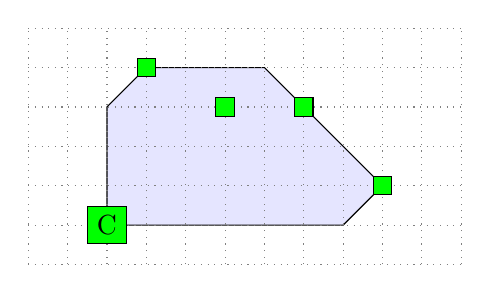
\begin{tikzpicture}[scale=0.5]
    %\draw[fill=red!10] (0,6) -- (0,0) -- (2,4) -- cycle;
    \draw[fill=blue!10] (2,1) -- (2,4) -- (3,5) -- (6,5) -- (9,2) -- (8,1) -- cycle;
    %\draw[fill=yellow!10] (3,6) -- (3,5) -- (6,1) -- (6,2) 
      -- cycle;
    %\draw[fill=green!10] (7,6) -- (12,6) -- (10,4) -- (5,4) 
      -- cycle;
    %\draw[fill=orange!10] (12,4) -- (11,0) -- (12,0) -- cycle;
    \draw[color=gray, style=dotted] (0,0) 
      grid[xstep=1cm, ystep=1cm] (11cm,6cm);
  	\node at (2,1) [draw,fill=green] {C};
  	%\node at (1.5,0.5) [draw=none]	 {C};
  	%\node at (9.5,1.5) [draw=none]	 {D};
  	\node at (3,5) [draw,fill=green] {};
  	\node at (9,2) [draw,fill=green] {};
  	\node at (7,4) [draw,fill=green] {};
  	\node at (5,4) [draw,fill=green] {};
  \end{tikzpicture}
  \caption{The octagonal hull of green points. The green point marked with the letter $C$ is a {\em corner} of the octagon hull.}
  % Clearly intersection with lines will be segments of lines. }
  \label{expotential}
  \end{center}
%  \end{figure}
\end{wrapfigure}
In the next two Sections we will obtain an upper bound of $586$ and respectively $485$ moves for Morpion 5T game solving \theoctagons instances of the linear problem (\ref{lp0})---(\ref{lp4}) described in Section \ref{linear}.  The following Theorem shows that the penalty, measured in extra potential, paid for solving such problems only on octagonal hulls is relatively small. In turn, thanks to Lemma \ref{lem:octagons}, the bound on the potential allows to limit the size of octagons. Thus we can focus attention on \theoctagons relatively small octagonal instances of linear programs. The number \theoctagons will be deduced in Theorem \ref{thm:octagons_in_o} later in this Section.

\begin{theorem}
\label{thm:octagonalization}
Let $G$ be a Morpion 5T position graph.
\begin{enumerate}
  \item  If $\hull G$ does not contain any corner, then
  \[
    \pot(\hull(G)) \leq \pot(G)
  \]
  \item If it does not contain opposite corners, then   \[
    \pot(\hull(G)) \leq \pot(G)+2
  \]
  \item If it contains at least two opposite corners, then
  \[\pot(\hull(G)) \leq \pot(G)+4.
 \]   
 Let $\modifier(\hull(G))$ by equal to $0,2,4$ like in the three above cases. 
\end{enumerate}
\end{theorem}

\noindent
We postpone the proof of Theorem~\ref{thm:octagonalization} until Section \ref{geometry}.

\subsection{The set of boards}

In this Subsection we describe a set of octagonal boards that contain every possible Morpion 5T position. As this set is  quite large, we will use symmetry to limit its size.

%\todo{Make a picture of the potential with enumeration of the edges}

  \begin{figure}[H]
  \begin{center}
  \begin{tikzpicture}[scale=0.35,>=stealth',thick]
  
  
    \begin{scope}[shift={(-4cm,0cm)}]
          \draw[fill=blue!10] (2,1) -- (2,4) -- (3,5) -- (6,5) -- (9,2) -- (8,1) -- cycle;
    	\draw[color=gray, style=dotted] (0,0) 
      grid[xstep=1cm, ystep=1cm] (11cm,6cm);
      
    
  		\node(place) at (6,5) [draw=none] {};
		\foreach \i in {1,2,3} 
		{
			\node(place) [draw,fill=yellow]  at ($(place)+(-1,0)$)  {};
        	\foreach \x / \y in {-1 / 1, 0 / .9, 1 / 1} 
			{
				\path(place) [->] edge node {} ($(place)+(\x,\y)$);
			}
		}
    \end{scope}
        

    
    \begin{scope}[shift={(8cm,0cm)}]
    \draw[fill=blue!10] (2,1) -- (2,4) -- (3,5) -- (6,5) -- (9,2) -- (8,1) -- cycle;
    \draw[color=gray, style=dotted] (0,0) 
      grid[xstep=1cm, ystep=1cm] (11cm,6cm);
      
    
  	\node(place) at (9,2) [draw=none] {};
	\foreach \i in {1,2,3} 
	{
		\node(place) [draw,fill=red]  at ($(place)+(-1,0)$)  {};
		\path(place) [->] edge node {} ($(place)+(.9,.9)$);
        \node(place) [draw,fill=red]  at ($(place)+(0,1)$)  {};
        \foreach \x / \y in {1 / 0, 1 / 1, 0 / 1} 
		{
			\path(place) [->] edge node {} ($(place)+(\x,\y)$);
		}
	}
    \end{scope}
    
    \begin{scope}[shift={(20cm,0cm)}]
        \draw[fill=blue!10] (2,1) -- (2,4) -- (3,5) -- (6,5) -- (9,2) -- (8,1) -- cycle;
    	\draw[color=gray, style=dotted] (0,0) 
      grid[xstep=1cm, ystep=1cm] (11cm,6cm);
      
    
  		\node(place) at (9,2) [draw=none] {};
		\foreach \i in {1} 
		{
			\node(place) [draw,fill=green]  at ($(place)+(-1,0)$)  {};
			\path(place) [->] edge node {} ($(place)+(.9,-.9)$);
        	\node(place) [draw,fill=green]  at ($(place)+(1,0)$) {};
        	\foreach \x / \y in {0 / -1, 1 / 0, 1 / -1} 
			{
				\path(place) [->] edge node {} ($(place)+(\x,\y)$);
			}
		}
    \end{scope}
    
    \begin{scope}[shift={(-4cm,-7cm)}]
        \draw[fill=blue!10] (2,1) -- (2,4) -- (3,5) -- (6,5) -- (9,2) -- (8,1) -- cycle;
    	\draw[color=gray, style=dotted] (0,0) 
      grid[xstep=1cm, ystep=1cm] (11cm,6cm);
      
    
  		\node(place) at (9,1) [draw=none] {};
		\foreach \i in {1,2,3,4,5,6} 
		{
			\node(place) [draw,fill=orange]  at ($(place)+(-1,0)$)  {};
        	\foreach \x / \y in {-1 / -1, 0 / -.9, 1 / -1} 
			{
				\path(place) [->] edge node {} ($(place)+(\x,\y)$);
			}
		}
    \end{scope}
    
    
    \begin{scope}[shift={(8cm,-7cm)}]
        \draw[fill=blue!10] (2,1) -- (2,4) -- (3,5) -- (6,5) -- (9,2) -- (8,1) -- cycle;
    	\draw[color=gray, style=dotted] (0,0) 
      grid[xstep=1cm, ystep=1cm] (11cm,6cm);
      
    
  		\node(place) at (2,0) [draw=none] {};
		\foreach \i in {1,2,3} 
		{
			\node(place) [draw,fill=gray]  at ($(place)+(0,1)$)  {};
        	\foreach \x / \y in {-1 / -1, -.9 / 0, -1 / 1} 
			{
				\path(place) [->] edge node {} ($(place)+(\x,\y)$);
			}
		}
    \end{scope}
    
    \begin{scope}[shift={(20cm,-7cm)}]
        \draw[fill=blue!10] (2,1) -- (2,4) -- (3,5) -- (6,5) -- (9,2) -- (8,1) -- cycle;
    	\draw[color=gray, style=dotted] (0,0) 
      grid[xstep=1cm, ystep=1cm] (11cm,6cm);
      
    
  		\node(place) at (2,4) [draw=none] {};
		\foreach \i in {1} 
		{
			\node(place) [draw,fill=cyan]  at ($(place)+(1,0)$)  {};
			\path(place) [->] edge node {} ($(place)+(-.9,.9)$);
        	\node(place) [draw,fill=cyan]  at ($(place)+(-1,0)$) {};
        	\foreach \x / \y in {-1 / 0, 0 / 1, -1 / 1} 
			{
				\path(place) [->] edge node {} ($(place)+(\x,\y)$);
			}
		}
    \end{scope}
    
    \begin{scope}[shift={(8cm,-14cm)}]
        \draw[fill=blue!10] (2,1) -- (2,4) -- (3,5) -- (6,5) -- (9,2) -- (8,1) -- cycle;
    	\draw[color=gray, style=dotted] (0,0) 
      grid[xstep=1cm, ystep=1cm] (11cm,6cm);
      
    
  		\node(place) at (2,1) [draw,fill=black] {};
        \path(place) [->] edge node {} ($(place)+(1,-1)$);
        \path(place) [->] edge node {} ($(place)+(0,-1)$);
  		\node(place) at (2,4) [draw,fill=black] {};
        \path(place) [->] edge node {} ($(place)+(-1,-1)$);
  		\node(place) at (3,5) [draw,fill=black] {};
        \path(place) [->] edge node {} ($(place)+(-1,0)$);
  		\node(place) at (6,5) [draw,fill=black] {};
        \path(place) [->] edge node {} ($(place)+(-1,1)$);
  		\node(place) at (9,2) [draw,fill=black] {};
        \path(place) [->] edge node {} ($(place)+(0,1)$);
        \path(place) [->] edge node {} ($(place)+(1,1)$);
  		\node(place) at (8,1) [draw,fill=black] {};
        \path(place) [->] edge node {} ($(place)+(1,0)$);
    \end{scope}
  \end{tikzpicture}
  \caption{The octagon $(3,3,0,1,6,0,3,1)$.The top 6 figures represent potential associated with $3a_1=3\cdot 3 = 9$, $4a_2=4\cdot 3=12$, $4a_4=4\cdot 1 = 4$, $3a_5=3\cdot 6$, $3a_7=3\cdot 3=9$, $4a_8=4\cdot 1=4$. The bottom figure represents missing $8$ edges of the potential. }
  \label{potential_dist}
  \end{center}
  \end{figure}

We say that a graph $G$ is \emph{non-degenerated} if it contains three vertices that are not on a single diagonal line.

\begin{lemma}\label{lem:octagons}
  Let $G$ be a non-degenerated octagon with edges of length $a_1, a_2, a_3, a_4$, $a_5, a_6, a_7, a_8$ with $a_1$ denoting the length of the top edge.
  The following equations hold.
  \begin{equation}
  	\tag{O1}
    \label{o1}
    \pot(G) = 8 + 3a_1+4a_2+3a_3+4a_4+3a_5+4a_6+3a_7+4a_8. 
  \end{equation}
  \begin{equation}
  	\tag{O2}
    \label{o2}
    a_8 = a_2 + a_3 + a_4 - a_7 - a_6. 
  \end{equation}
  \begin{equation}
  	\tag{O3}
    \label{o3}
    a_1 = a_4 + a_5 + a_6 - a_8 - a_2. 
  \end{equation}
  If $G$ contains the starting cross of Morpion 5T game, then
  \begin{equation}
  	\tag{O4}
    \label{o4}
    a_1 + a_2 + a_ 3 \geq 10 
  \end{equation}
  \begin{equation}
  	\tag{O5}
    \label{o5}
    a_8 + a_1 + a_ 2 \geq 10 
  \end{equation}
  \begin{equation}
  	\tag{O6}
    \label{o6}
    a_2 + a_3 + a_4 \geq 10 
  \end{equation}
  Using rotation by multiple of $90$ degrees and a reflection along the $y$-axis we can always obtain a graph that satisfies
  \begin{equation}
  	\tag{O7}
    \label{o7}
    a_1 \geq a_3, a_1 \geq a_5, a_1 \geq a_7 
  \end{equation}
  \begin{equation}
  	\tag{O8}
    \label{o8}
    a_8 \geq a_2
  \end{equation}
\end{lemma}
\begin{proof}
Condition (\ref{o1}) follows from distribution of potential visualized in Figure \ref{potential_dist}.
Conditions (\ref{o2}), (\ref{o3}) are elementary geometric properties of octagons. We will verify them on the example presented in Figure \ref{potential_dist}. Indeed, \[ a_8 = 1. \]
On the other hand \[ a_2+a_3+a_4-a_7-a_6=3+0+1-3-1=1. \]
Similarly, \[ a_1 = 3 \]
and \[ a_4+a_5+a_6-a_8-a_2=1+6+0-1-3=3. \]

Properties (\ref{o4}),(\ref{o5}),(\ref{o6}) follows from the observation that in order to embed the starting cross of Morpion 5T (see Figure \ref{fig:rules}), the projections of the octagon in diagonal, horizontal and vertical directions must be of length at least $10$. 

Property (\ref{o7}) can be guaranteed through rotation by a multiple of $90$ degrees. Then 
property (\ref{o8}) can be guaranteed through reflection along the $y$--axis. This reflection preserves property (\ref{o7}).
\end{proof}

\begin{theorem}
\label{thm:octagons_in_o}
  Let $\mathcal{O}$ denote the set of octagons $O$ that satisfy constraints (\ref{o1}) --- (\ref{o8}) of Lemma~\ref{lem:octagons} and the constraint given by the equality $\pot(O) = 288 + \modifier(O)$.
  The number of elements of $\mathcal{O}$ is \theoctagons and the octagon with the largest number of vertices is an equilateral octagon with sides of length $10$. This octagon contains $741$ vertices.
\end{theorem}


\begin{proof} %(of Theorem \ref{thm:octagons_in_o}) 
Every octagon $O$ with $\pot(O) < 288 + \modifier(O)$ is included in an octagon $O'$ with $\pot(O') = 288 + \modifier(O')$. Hence we can ignore in our calculations octagons with $\pot(O) < 288 + \modifier(O)$.
The number of relevant octagons calculated using the script {\tt octagons.cpp} (see the repository \cite{thewebpage}). The script generates all instances of octagons satisfying constraints of this Theorem. %\todo{Let us make sure that this is the right name.}
\end{proof}

\noindent
As a corollary we obtain the bound presented in \cite{demaine}.
%, without appealing to the Brass formula.
\begin{corollary}[\cite{demaine}]
  The number of moves in a Morpion 5T game is bounded by $705$.%\todo{It is also valid for Morpion 5T++? A claim like this is currently in the introduction.}
\end{corollary}
\begin{proof} We list all octagons in ${\mathcal O}$ and check how many dots can placed in a fixed octagon, given the starting $36$ dots. The best result consists of $705$ new dots for the equilateral octagon with sides of length $10$.\footnote{This proof does not rely on linear optimization. We just go over a finite list of octagons.}
\end{proof}

\noindent
Let us notice, that this Corollary is weaker than the one obtained in \cite{demaine}, because the above method applies to Morpion 5T, but not to Morpion 5T++ game. 

%\todo{Figure: distribution of areas, whatever it means}